\documentclass[12pt,letterpaper]{article}
\usepackage[spanish]{babel}
\usepackage[utf8]{inputenc}
\usepackage[right=3cm,left=3cm,top=2cm,bottom=2cm,headsep=0cm,footskip=0.5cm]{geometry}
\usepackage[dvips]{graphicx}
\usepackage{verbatim}
\usepackage{multicol}
\usepackage{fancyvrb,relsize}
\usepackage{amsthm}
\usepackage{amssymb}
\usepackage{listings}
\usepackage{wrapfig}
\usepackage{subfig}
\usepackage{placeins}
\usepackage{setspace}
\usepackage{amsmath}

\begin{document}
\begin{titlepage}
\begin{figure}[ht]

\includegraphics[scale=1]{logo_departamento.eps}
\label{DCC}
\vspace{1cm}
\end{figure}
\begin{center}
\vspace{4cm} {\Huge Tarea 2: Planificación de Trabajos}

\vspace{1cm} {\Large CC4102 - Diseño y Análisis de Algoritmos}
\vspace{7.5cm}
\end{center}

\begin{tabbing}
\hspace*{7cm}\=\hspace*{3.5cm}\= \kill

\> {\large Profesor:} 	\> 	{\large Gonzalo Navarro} \\ \\
\> {\large Auxiliar:}	\> 	{\large Teresa Bracamonte} \\ \\
\> {\large Alumnos:}	\> 	{\large Cristián Carreño} \\ \\
\> {\large } 			\> 	{\large Sergio Maass} \\ \\
\> {\large Fecha:} 		\> 	{\large 17 de Noviembre de 2013}
\end{tabbing}

\end{titlepage}
%\begin{doublespace}

%\tableofcontents
\newpage

\section{Introducción}
	Los algoritmos online cumplen un rol muy importante al permitir resolver problemas a medida que su entrada se va recibiendo, o sea, sin conocer el total de los datos previamente. Pero además, son muy útiles para aproximar soluciones a problemas difíciles en tiempo razonablemente corto. \\
	
	Diversos problemas de optimización pertenecientes a la clase $NP$ admiten soluciones aproximadas mediante algoritmos online $p$-competitivos. Un algoritmo de estas características permite resolver instancias arbitrarias del problema en tiempo polinomial, garantizando que la solución estará dentro de un radio $p$ del óptimo. Esto es muy importante, ya que si $P \not= NP$ -lo que parece ser el caso- no es posible encontrar una solución óptima en tiempo polinomial. \\
	
	En este informe se presentarán dos versiones del problema de planificación de trabajos ($NP-completo$\footnote{Garey, M.R. (1976). "The Complexity of Flowshop and Jobshop Scheduling"}) y se diseñará un algoritmo online 2-competitivo para cada una. Se demostrará formalmente la competitividad de cada algoritmo y luego se comprobará experimentalmente.

\section{Trabajos de una etapa}
	El problema consiste en un conjunto de $n$ trabajos que deben asignarse a $m$ máquinas idénticas. Cada trabajo $j$ requiere una cantidad de tiempo $T_{j}$ para ser finalizado. Además, cada trabajo $j$ sólo puede ser asignado a una máquina $A_{j}$, y debe ejecutarse por completo y sin interrupciones en esta.\\
	
Sea $A$ una asignación de trabajos a máquinas, y sea el $makespan$ definido por: $makespan(A) = max_{i} \sum_{A_{j}=i} T_{j}$. El objetivo del problema es determinar la asignación $A$ que minimiza el $makespan$.

\subsection{Algoritmo 2-competitivo propuesto}
\label{sec:prop-alg1}
	El algoritmo consiste simplemente en asignar cada trabajo $j$ a la máquina que posea la menor carga. En particular, para cada $j$:
\begin{itemize}
\item[1.] Obtener la máquina $M_{i}$ de menor carga $L_{i}$.
\item[2.] Asignar $j$ a $M_{i}$
\item[3.] $L_{i} := L_{i} + T_{j}$
\end{itemize}

	La complejidad del algoritmo depende del paso 1. Usando un $heap$ podemos obtener la máquina de menor carga en tiempo $O(1)$ y luego reinsertarla en la estructura con su nueva carga en tiempo $O(\log{m})$. Por lo tanto, para $n$ trabajos tenemos un tiempo $O(n \log{m})$.

\subsection{Demostración de competitividad}
	Sea $L_{i}$ la carga de la máquina con mayor tiempo asignado, y sea $j$ su último trabajo. La carga de la máquina antes de esa asignación era $L_{i} - T_{j}$. Debido a que el algoritmo asigna un trabajo a la máquina de menor carga tenemos que $L_{i} - T_{j} \leq L_{k}, \forall k \in [1, m]$. \\
	
	Luego, sumando sobre todas las máquinas obtenemos
	
\begin{eqnarray}
L_{i} - T_{j}	&\leq& 		\frac{1}{m} \sum_{k=1}^{m} L_{k}	\nonumber \\
				&=& 		\frac{1}{m} \sum_{k=1}^{n} T_{k}  	\nonumber \\
				&\leq& 		L^{*} \label{eq:1}
\end{eqnarray}

Donde $L^{*}$ corresponde al $makespan$ del caso óptimo.\\

Finalmente, considerando (\ref{eq:1}) y el hecho de que $T_{j} \leq L^{*}$, ya que el trabajo más largo igual debe ser realizado por alguna máquina en el caso óptimo, tenemos que 

\begin{eqnarray}
L_{i}		&=&		L_{i} - T_{j} + T_{j}	\nonumber \\
			&\leq&	L^{*} + T_{j} 			\nonumber \\
			&\leq& 2 L^{*}
\end{eqnarray}

Con lo que se demuestra que el $makespan$ obtenido por el algoritmo online está acotado por el doble del $makespan$ en el caso óptimo. O sea, el algoritmo es 2-competitivo.

\subsection{Comprobación empírica de competitividad}
	Para comprobar empíricamente la competitividad del algoritmo propuesto, éste se implementó en Java junto a un algoritmo que encuentra el makespan óptimo para este problema. Luego se hicieron pruebas con ambos algoritmos, usando los mismos datos, y se compararon los makespan obtenidos.

\subsubsection{Implementación del algoritmo online}
	El algoritmo online se implementó tal cual fue descrito en la sección \ref{sec:prop-alg1}. Se utilizó la clase $PriorityQueue$ de $java.utils$, la cual está implementada con un $heap$, para almacenar las máquinas ordenadas según carga. De este modo, se pueden planificar $n$ tareas en $m$ máquinas en tiempo $O(n \log{m})$.

\subsubsection{Implementación del algoritmo óptimo}
	Para obtener la asignación de una lista $L$ de $n$ trabajos a $m$ máquinas que produce un menor makespan, se procedió a generar todas las posibles asignaciones que pueden entregar distinto makespan. Para esto se utilizó un arreglo $A$ de tamaño $n$ donde cada índice $i \in [0, n-1]$ representa un trabajo, y cada valor $A_{i}$ representa la máquina que se le ha asignado al trabajo $i$. Además se utilizó un objeto $G$ encargado de generar asignaciones para $A$ a través de su método $G.nextAssignment()$, y de señalar mediante un método $G.hasNext()$ si siguen habiendo asignaciones para generar. El algoritmo funciona del siguiente modo:
	
\begin{itemize}
\item Se comienza con $A$ con todas sus entradas en cero.
\item Se inicializa el entero $minMakespan := Integer.MAX\_INT$
\item Mientras $G.hasNext()$ entregue verdadero:
	\begin{itemize}
	\item Se asigna $A' := G.nextAssignment()$.
	\item Se prueba la asignación $A'$ con la lista $L$ y $m$ máquinas y se calcula su $makespan$.
	\item Si $makespan(A') < minMakespan$:
		\begin{itemize}
		\item Se copia $A'$ en $A$. 
		\item $minMakespan := makespan(A')$.
		\end{itemize}
	\end{itemize}
\item Ahora $A$ contiene la asignación que minimiza el makespan.
\end{itemize}
	
	 El objeto $G$ mantiene un arreglo $B$ interno que va modificando para producir cada asignación. $B$ se inicializa con todas sus entradas en $0$, representando que todos los trabajos son asignados a la máquina $0$. $G.nextAssignment()$ opera del siguiente modo:

\begin{itemize}
\item Se itera desde $i = n-1$ hasta $i = 0$:
	\begin{itemize}
	\item Si $i = 0$, desde ahora $G.hasNext()$ siempre retornará falso. Se sale del ciclo.
	\item Si $B_{i} + 1 < m$, se asigna $B_{i} := B_{i} + 1$ y se sale del ciclo.
	\item En otro caso, se asigna $B_{i} = 0$ y se continúa en el ciclo.
	\end{itemize}
\item Se retorna $B$, el cual representa una nueva asignación.
\end{itemize}

De esta forma se verifican todas las asignaciones posibles que comienzan asignándole el trabajo $0$ a la máquina $0$. No es necesario verificar otros casos ya que asignarle el primer trabajo a otra máquina no reducirá el makespan en ningún caso.\\

Este algoritmo genera $m^{n-1}$ asignaciones y para cada una de ellas el cálculo del makespan para una lista dada toma tiempo $O(n)$. Por lo tanto, el algoritmo tiene una complejidad de $O(nm^{n-1})$. Cabe destacar que este largo tiempo podría mejorarse asegurándose de no generar asignaciones equivalentes ([0 2 2 1] y [0 1 1 2] son equivalentes porque siempre entregarán el mismo makespan), y también podría paralelizarse para aprovechar las arquitecturas multicore. Sin embargo, lo que interesa en este trabajo es comparar los makespan obtenidos por este algoritmo con los que obtiene la versión online, y no cuánto se demore, por lo que se dejará así.

\subsubsection{Experimentos}
	Para comprobar la competitividad del algoritmo online se procedió a comparar los makespan que entrega con los que entrega el algoritmo óptimo para la misma lista de trabajos y número de máquinas. Para esto se generaron listas con trabajos de duración aleatoria entre 1 y 100, y se obtuvieron los makespan para las asignaciones encontradas por ambos algoritmos.

\subsubsection{Resultados}
	Se probó con listas de tamaño 8, 10, 12, 14 y 16, y 4 máquinas. Para cada tamaño de lista se produjeron 400 listas y se compararon los makespan obtenidos por ambos algoritmos.\\

\begin{figure}[ht]
\centering
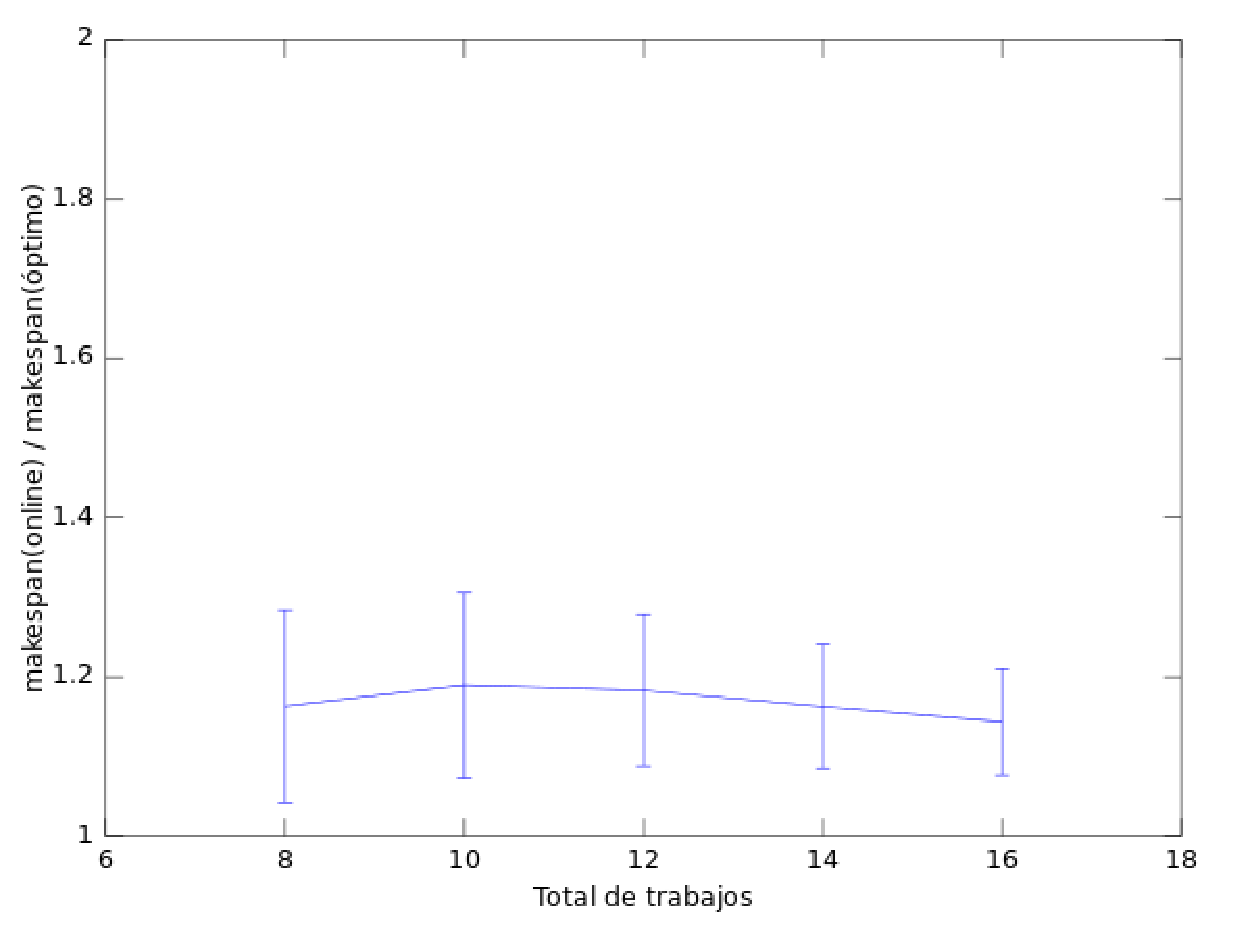
\includegraphics[scale=0.75]{fig1.eps}
\caption{Comparación de $makespan$ entre algoritmo online y algoritmo óptimo en función del número de trabajos, con 4 máquinas. Cada punto representa la media entre 400 datos, y las barras son la desviación estándar.}
\label{fig:1}
\end{figure}

En la figura \ref{fig:1} se observa que los makespan obtenidos por el algoritmo online fueron mayores a los obtenidos por el algoritmo óptimo en un factor bastante menor a 2, que es la cota teórica calculada. Esta razón tiende a disminuir en promedio, y con desviaciones estándar cada vez más acotadas, a medida que se incrementa el número de trabajos.\\

Luego se realizó otra prueba similar pero variando el número de máquinas en vez del número de trabajos. Los resultados de este experimento se graficaron en la figura \ref{fig:2}.

\begin{figure}[ht]
\centering
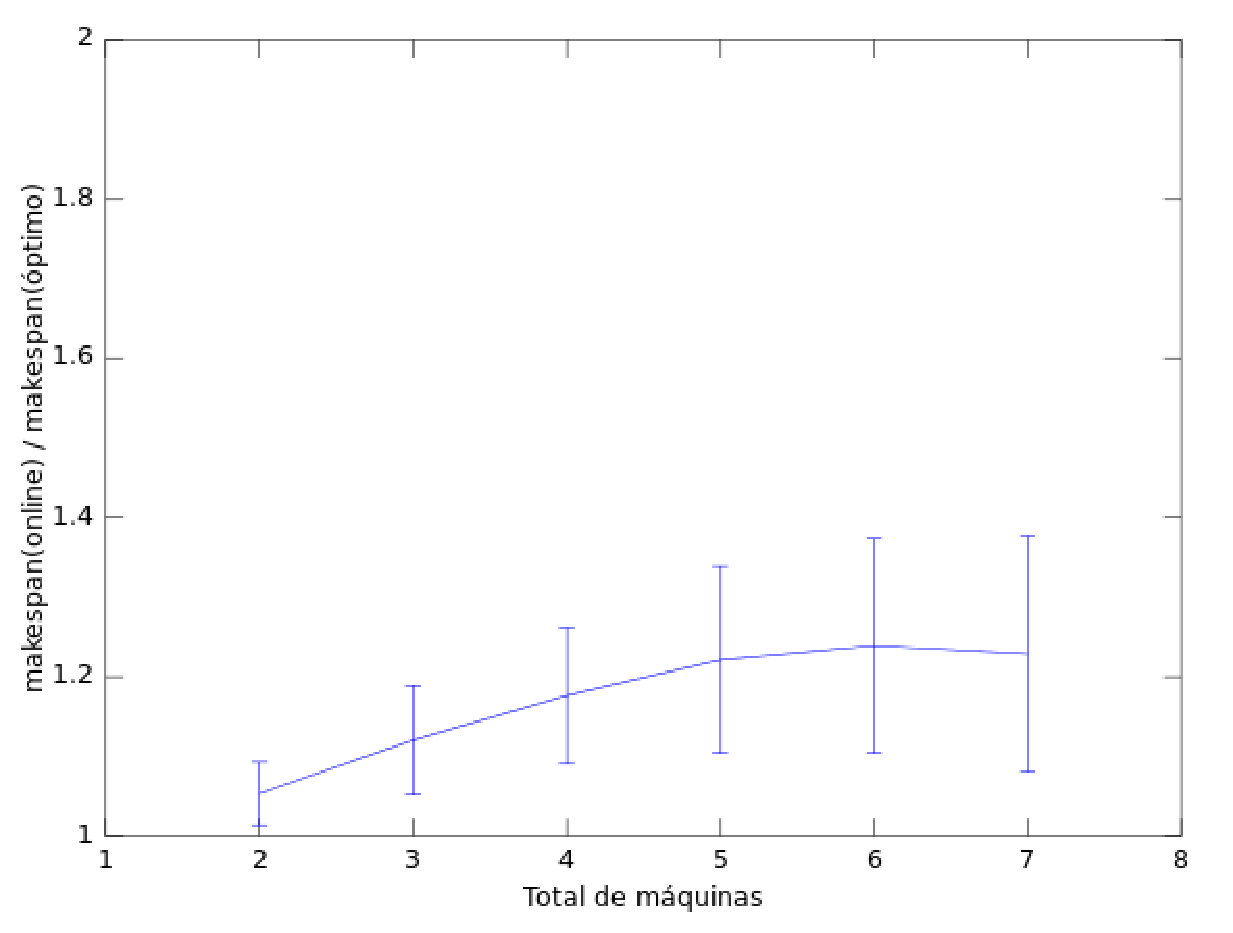
\includegraphics[scale=0.75]{fig2.eps}
\caption{Comparación de $makespan$ entre algoritmo online y algoritmo óptimo en función del número de máquinas, con 12 trabajos. Cada punto representa la media entre 400 datos, y las barras son la desviación estándar.}
\label{fig:2}
\end{figure}

En la figura \ref{fig:2} se observa que al aumentar el número de máquinas la razón $\frac{makespan(online)}{makespan(optimo)}$ crece hasta alcanzar un máximo en $\frac{m}{2} = 6$ máquinas y luego comienza a disminuir. La disminución a partir de ese punto no es muy evidente debido al margen de error y a que sólo se realizó el experimento hasta 7 máquinas (debido al tiempo que tomaba calcular para $m \geq 8$), sin embargo tiene sentido ya que a medida que el número de máquinas se acerca al número de trabajos estas van quedando más desocupadas hasta que a cada máquina le toca exáctamente un trabajo, cuando $m = n$, con lo que $\frac{makespan(online)}{makespan(optimo)} = 1$. Por otra parte, se observa que incluso en el punto máximo, y considerando el margen de error, el rendimiento del algoritmo online con respecto al óptimo está considerablemente por debajo de la cota teórica de 2 calculada. \\

Extrapolando estos resultados podemos afirmar que el rendimiento del algoritmo online con respecto al óptimo suele ser bastante mejor que el peor caso teórico cuando procesa trabajos de duración aleatoria. Este rendimiento tiende a mejorar lentamente a medida que se incrementa el número de trabajos, y tiende a reducirse a medida que aumentan las máquinas hasta alcanzar un máximo en $m/2$, a partir de donde mejora progresivamente hasta igualar al óptimo en $m = n$.

\section{Trabajos con múltiples etapas}
\subsection{Algoritmo 2-competitivo propuesto}
\subsection{Demostración de competitividad}
\subsection{Comprobación empírica de competitividad}
\subsubsection{Implementación del algoritmo online}
\subsubsection{Implementación del algoritmo óptimo}
\subsubsection{Experimentos}
\subsubsection{Resultados}

\section{Conclusiones}

%\end{doublespace}
\end{document}